%
% Author: Antigoni Kourou
%
\let\textcircled=\pgftextcircled
\chapter{Results}
\label{chap:res}
\section{Overview of sentiment scores}
Sentiment analysis and feature extraction from text reviews of Airbnb feedback system provides us with a set of discrete estimators of customer opinions per sentence, referred as sentiment scores (SS). Each listing in the dataset has in average 25.1 reviews, each of them consisting of 5.1 sentences in average. In total there are 12 798 negative sentences, with sentiment lower than 0, and 236 904 positive ones, meaning that the number of positive sentences is 18.5 times higher than the number of the negative ones.  This fact is visualized in Figure \ref{fig:sent}a, which shows the sentences sort in ascending order by their SS. In addition, Figure \ref{fig:sent}b shows the normalized frequencies of the SS round by 1. From the graph can be noticed that the most frequent SS are 0, 0.6 and 0.8. The presence of two relatively high SS indicates once again the tendency of reviewers to express positive emotions. On the other hand, the presence of so many sentences with 0 sentiment is an interesting observation and it will be discussed in the following section. In addition, the graphical presentation of normalized frequencies, excluding the sentences with no-sentiment, reveals a J-shaped distribution, suggested earlier in the literature \cite{hu2009overcoming}. The tendency of SS to avoid the "slightly" negative or positive zones around 0 has two probable explanations. First, text reviews are mostly used by customers to express their strong sentiments \cite{hu2009overcoming, pavlou2006nature}, and second, the pipeline may fail in identifying the SS of sentences with slight sentiment.
\begin{figure}[h!]
\centering
	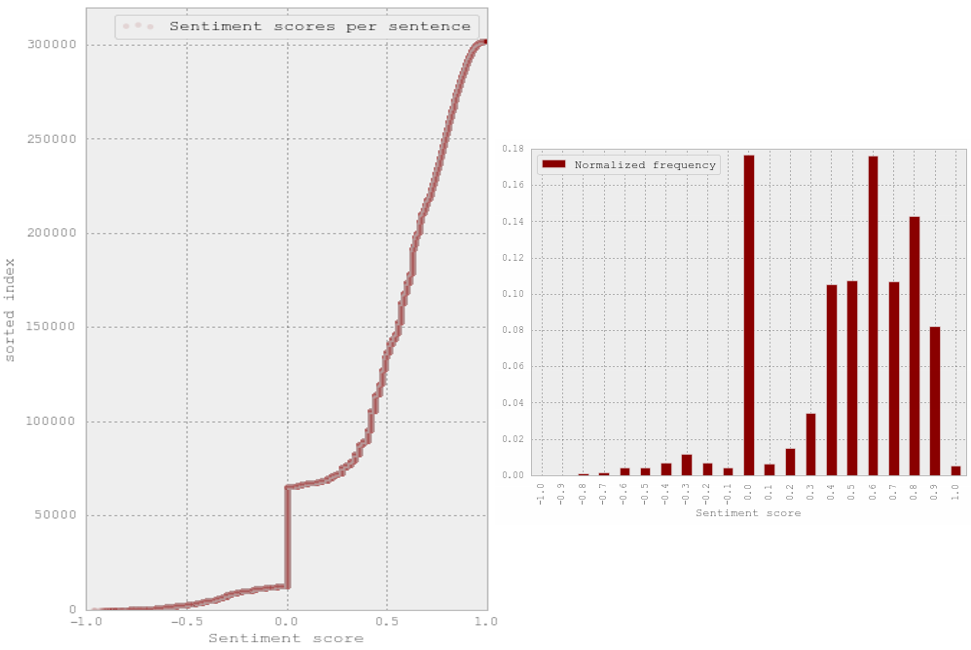
\includegraphics[height=0.35\textheight]{normalized_sentiment_freq}
% * <antigoni.kourou@student.uva.nl> 2016-06-14T10:59:51.526Z:
%
% How to draw a normal distribution curve for the normalized frequencies?
%
% ^.
	\caption{Sentiment scores of each sentence of reviews in the dataset}
	\label{fig:sent}
\end{figure}
Another level of analysis is to group the SS by accommodation features. The distributions of their SS per sentence are visualized and compared. From this comparison, it is noticed that the most frequent SS per sentence differ from one feature to the other, meaning that some features tend to be systematically rated higher than the others. This part of analysis, including their descriptions and visualizations can be found in Appendix I.
%
%
% ------------------ NO SENTIMENT -----------------
%
\section{The case of sentences with "no sentiment"}
%
%
As it is noticed in Figure \ref{fig:sent}, the SS of many sentences is equal to 0. From a deeper point of view results that 17.3\% of the total sentences have no-sentiment. This phenomenon is thought to have three possible explanations. First, it can be the case of booking cancellations. Every time that a host cancels the reservation, an automatic message is posted by the Airbnb system as a review of the guest-to-be. These messages are considered by the pipeline as reviews with no-sentiment and they are found in 1259 cases. The occurrence of cancellations is checked for each listing and from the analysis we could retrieve the listings with the highest number of cancellations. A host who has canceled 27 times seems to be on top of the list, however the mean number of cancellation per listing is 1.7. In total 32.7\% of the hosts have canceled at least once the reservation, meaning that the customers should  have to pay attention to these cases. A second explanation for the presence of no-sentiment sentences is that the pipeline fails to identify their sentiment. Thirdly,  it can be the case when the sentence has indeed neutral sentiment. Since we are not able to identify for every sentence if it is an error of the pipeline or an actual neutral value, the case of sentences with sentiment zero are excluded from the following analysis, in order not to affect the average sS per review or per listing.

\section{Most mentioned features}
An interesting point of view is the analysis of most mentioned features in the comments, which is done in three granularity levels: sentence level, review level and listing level. For all the three levels, we can clearly see that \textit{location} is the most mentioned feature by reviewers of Airbnb and \textit{check-in} is the least mentioned one. From this comparison, Figure \ref{fig:fea}, we can indicate that the frequency of features is more accurate in review level, because we make sure that the opinions of each reviewer are treated equally and they generate only one average sentiment score per feature. Measuring the frequencies in sentence level would weight the opinion of some reviewers more than others. Similarly, in listing level it would take at least one sentence to indicate that the feature is mentioned in the listing, which produces over-estimated frequency values per feature. 
\begin{table}[h!]
\footnotesize 
\centering
\begin{tabular}{|m{2.1cm}|m{2.4cm}|m{2.6cm}|m{1.15cm}|}

\hline
\centering {\textbf{}}  & \centering {\textbf{Sentences}} & \centering {\textbf{Reviews}} & {\textbf{Listings}} \\

\hline
\centering {Accuracy}  & \centering {8364} & \centering {7915} &  {1773} \\ \hline

 \centering {Check-in} & \centering {5818} & \centering  {5454} & {1623}\\ \hline
 
 \centering {Cleanliness} & \centering {18440} & \centering {17757} & {2076}\\ \hline
 
\centering  {Communication} & \centering {16894} & \centering {14610} & {2067} \\ \hline

\centering {Location} & \centering {69616} & \centering {44539} & {2331}\\ \hline

\centering {Value} & \centering {19862} & \centering {18811} & {2145}\\ \hline
\end{tabular}
\caption{Number of sentences, reviews and listings where features are mentioned}
\label{res1}
\end{table}

\begin{figure}[h!]
\centering
	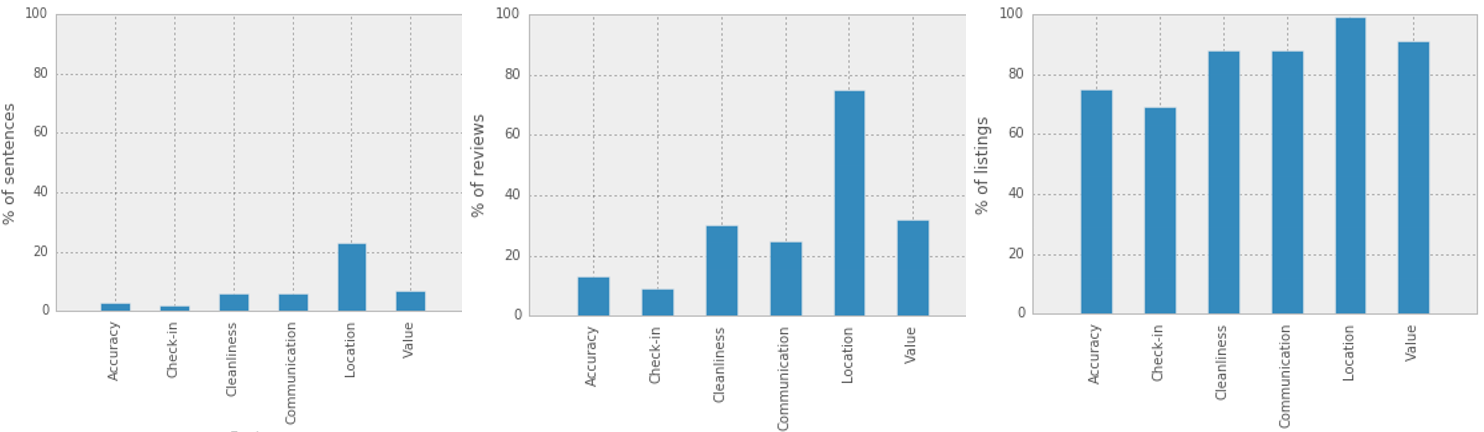
\includegraphics[height=0.2\textheight]{feature_mentioned}
	\caption{Percentage of sentences, reviews and listings where the features are mentioned}
	\label{fig:fea}
\end{figure} 
%
%
%
\section{The trade-off between sentiment and number of reviews}
%
%
\begin{figure}[h!]
	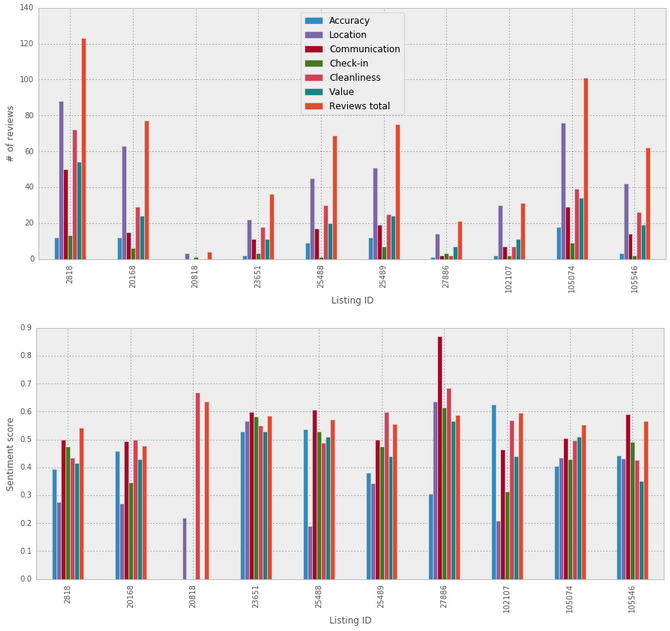
\includegraphics[height=0.75\textheight]{features_sentiment}
	\caption{Features mentioned in review level per each listing and their sentiment}
	\label{fig:feasent}
\end{figure}
Figure \ref{fig:feasent}a) shows for 10 random listings the number of reviews mentioning each of the features, as well as their total number of reviews. It is logical that we (as a customer) always prefer listings, which have many reviews, so their SS would be reliable. Therefore, under this assumption, it is important to compare not only the total number of reviews with the SS of the listing, but also the number of reviews per feature with the corresponding SS of that feature. The second part of Figure \ref{fig:feasent} shows exactly, for the same 10 random listings, the SS of each feature and the overall SS of the listing based on its reviews. The graphs are placed underneath each other in order to compare the SS per feature with the number of reviews for each of them. For example, from Figure \ref{fig:feasent}, we can see that for the listing with ID 22886, even though it has the highest sentiment score on \textit{communication}, only a very few people have commented on it compared to the other listings. Therefore, its SS is not very reliable and each customer would have to make an individual choice between the listings, depending on the number of reviews per feature and the corresponding SS of the features of their interest. 

\section{Pipeline ratings compared to Airbnb stars}
In this paper, it is stated the importance of comparing the pipeline generated SS with the Airbnb's quantitative data. In the Airbnb feedback system, the customers can check the number of reviews for a listing, the overall average rating, revealed after the first three reviews and the average rating of the six specific features: \textit{accuracy, check-in, cleanliness, communication, location, value}. The SS of the pipeline are converted to stars following the scheme mentioned in Chapter \ref{chap:prop}. Then the ratings are compared in listing and feature level. 
\subsection{Overall stars per listing}
\label{overallstars}
%
\begin{wrapfigure}[15]{r}{8cm}
\centering
	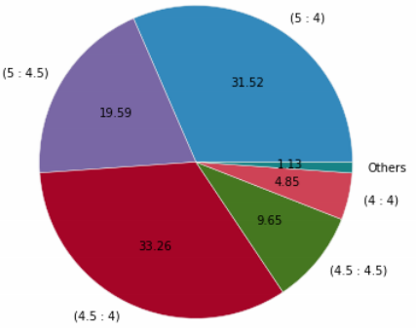
\includegraphics[height=0.27\textheight]{star_combinations}
	\caption{Comparison of combinations Airbnb and pipeline stars per listing}
	\label{fig:comb1}
\end{wrapfigure}
%
The results of overall ratings between Airbnb and pipeline show that both sets are very similar in general, however several differences exist. In both datasets, there is no listing with negative sentiment, meaning lower than 3 stars. All the possible combinations of values are retrieved from the dataset and they are visualized in Figure \ref{fig:comb1}. The most common combinations are (5:4),(5:4.5) and (4.5:4), where the first value stays for Airbnb rating and the second for the pipeline. This comparison shows that in 84.6\% of the cases, the ratings of Airbnb are higher than ratings generated from the text feedback. The between the values are presented in Table \ref{res2}, from where we see that 53.7\% of cases have half a star difference, 31.5\% of cases have one star difference and only 0.14\% of the cases have a difference higher than one star (4 cases explicitly). 
%
\begin{wraptable}[8]{l}{8cm}
\footnotesize 
\centering
\begin{tabular}{|m{2cm}||m{2cm}|m{1cm}|}

\hline
\centering {\textbf{Difference}}  & \centering {\textbf{Frequency}} & {\textbf{\%}} \\

\hline
\centering {\textbf{0.5}}  & \centering {1097}  &  {52.9} \\ \hline

 \centering {\textbf{1.0}} & \centering {654} & {31.5}\\ \hline
 
 \centering {\textbf{0.0}} & \centering {301} & {14.5}\\ \hline
 
\centering  {\textbf{-0.5}} & \centering {17} & {0.8} \\ \hline

\centering {\textbf{1.5}} & \centering {3} & {0.1}\\ \hline

\centering {\textbf{-2.0}} & \centering {1} & {0.04}\\ \hline
\end{tabular}
\centering
\caption{Differences in overall stars}
\label{res2}
\end{wraptable}
The differences more than 1 stars are treated as isolated cases and they are checked individually. For example, in the case of 1 listing where the difference of the pipeline from Airbnb values is 2 stars (Figure \ref{fig:6.5}), the listing has actually only one review composed of one sentence. The high SS of this sentence makes the pipeline be mistaken for generating an accurate SS. Therefore, it is recommended to set a limit in the number of reviews, where the pipeline is based on generating the SS of a listing. This case will be treated separately in the following section.
\begin{figure}[h!]
\centering
	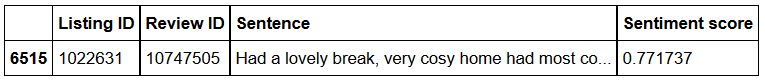
\includegraphics[height=0.06\textheight]{listing-2}
	\caption{Reviews of listing with (-2) stars difference}
	\label{fig:6.5}
\end{figure}

Statistically, the differences between values predicted by the pipeline and the  actual Airbnb values are measured using the RMSE. The RMSE of differences in overall ratings results to be 0.675, which confirms the presence of a certain bias between the two samples, as it is already stated.
\begin{equation}
\small
RMSE = \sqrt {{\frac{{\sum\limits_{{i = 1}}^n {{{\left( {{y_\textsubscript{i (Airbnb)}} - {{\hat{y}}_\textsubscript{i (Pipeline)}}} \right)}^2}} }}{{n}}}}
\label{RSMEresults}
\end{equation}
%
%
%
\subsection{Stars of features per listing}
\label{6.5.2}
In contrast to the results of comparing the overall ratings, the combinations of Airbnb and pipeline stars per feature appear less similar. Depending on the feature compared, new combinations in stars are present and the differences between the predicted stars and Airbnb values are bigger. Table \ref{res3} shows the differences in stars for 
%
%
\begin{wraptable}[13]{l}{7.7cm}
\footnotesize 
\centering
\begin{tabular}{|m{0.9cm}|m{0.9cm}|m{0.7cm}||m{0.9cm}|m{0.9cm}|m{0.7cm}|}

\hline
\multicolumn{3}{|c||}{\textbf{Feature:Accuracy}} & \multicolumn{3}{|c|}{\textbf{Feature:Cleanliness}} \\
\hline
\centering {\textbf{Diff.}}  & \centering {\textbf{Freq}} & {\textbf{\%}} & \centering {\textbf{Diff.}}  & \centering {\textbf{Freq}} & {\textbf{\%}}\\

\hline
\centering {\textbf{1.0}}  & \centering {649}  &  {41.2} & \centering {\textbf{0.5}}  & \centering {839}  &  {47.1}\\ \hline

 \centering {\textbf{0.5}} & \centering {571} & {36.9} &  \centering {\textbf{0.0}} & \centering {486} & {27.3}\\ \hline
 
 \centering {\textbf{0.0}} & \centering {162} & {1.4} & \centering {\textbf{1.0}} & \centering {286} & {16.1}\\ \hline
 
\centering {\textbf{1.5}} & \centering {105} & {6.7} & \centering  {\textbf{-0.5}} & \centering {111} & {6.2} \\ \hline

\centering {\textbf{-0.5}} & \centering {32} & {2.1} &  \centering {\textbf{-1.0}} & \centering {27} & {1.5}\\ \hline

\centering {\textbf{2.5}} & \centering {10} & {0.6} &  \centering {\textbf{1.5}} & \centering {22} & {1.2}\\ \hline

 \centering {\textbf{2.0}} & \centering {7} & {0.4} &  \centering {\textbf{2.0}} & \centering {6} & {0.3}\\ \hline
 
\centering  {\textbf{-1.0}} & \centering {6} & {0.3} &  \centering {\textbf{2.5}} & \centering {2} & {0.1} \\ \hline

\centering {\textbf{3.0}} & \centering {5} & {0.3} &  \centering {\textbf{-2.5}} & \centering {1} & {0.05}\\ \hline

\centering {\textbf{3.5}} & \centering {1} & {0.06} &  \centering {\textbf{-1.5}} & \centering {1} & {0.05}\\ \hline
\end{tabular}
\centering
\caption{Differences for two features}
\label{res3}
\end{wraptable}
two features, Accuracy and Cleanliness. From Table \ref{res3}, we see that for \textit{Cleanliness} the differences are mostly 0.5 stars, while for \textit{Accuracy} difference of 1 stars prevails. Furthermore, it is noticed that differences reach in some cases very high values, for example 3.0 or 3.5, meaning that the sentiment detected by the pipeline goes completely in another direction from Airbnb's. These cases can be either errors of prediction or cases when the pipeline successfully detects the hidden sentiment of features out of text reviews. To analyze the issue, the RMSE is calculated for each feature. Its values show that \textit{Location} is the feature with the lowest RMSE, while \textit{Checkin} is the feature with the highest one, 0.48 and 1.51 respectively.  These results align with the fact that \textit{location}is the most mentioned feature and \textit{Check-in} the least mentioned one (Section 6.2), which leads us to thinking that \textit{the more the feature is mentioned or the more reviews a listing has, the more similar the values of the pipeline are to Airbnb}. Thus, this assumption brings us again to the point where the  number of reviews for the pipeline to generate a rating should be limited. The following section deals explicitly with this issue.
%
%
%
\section{Conditional analysis on the number of reviews}
%
%
%
While comparing the ratings of Airbnb with the values predicted from the pipeline, we have concluded that the number of reviews is affecting the analysis. In this section, this assumption is tested in two levels: for the overall ratings and for each feature of the listing. In the first case, the pipeline is conditioned to generate a SS per listing only if that listing has more than 3 reviews (the same limit the Airbnb has set for calculating the system ratings). From this conditioning, results that the RMSE of overall ratings changes from 0.675 to 0.673, which is not a significant change. This means that the differences between Airbnb and pipeline ratings are not caused by isolated cases of listing with less than 3 reviews. On the contrary, as stated in \ref{overallstars}, the differences are the result of a systematic tendency of Airbnb values to be higher than the pipeline.
\begin{table}[h!]
\footnotesize 
\centering
\begin{tabular}{|m{2.1cm}|m{2.4cm}|m{2.6cm}|m{1.8cm}|}

\hline
\centering {\textbf{}}  & \centering {\textbf{RMSE }} & \centering {\textbf{RMSE AFTER}} & {\textbf{\# of RMSE}} \\

\hline
\centering {Accuracy}  & \centering {1.18} & \centering {0.8} &  {-0.38} \\ \hline

 \centering {Check-in} & \centering {1.52} & \centering  {0.92} & {-0.6}\\ \hline
 
 \centering {Cleanliness} & \centering {0.7} & \centering {0.55} & {-0.15}\\ \hline
 
\centering  {Communication} & \centering {0.68} & \centering {0.55} & {-0.13} \\ \hline

\centering {Location} & \centering {0.49} & \centering {0.46} & {-0.03}\\ \hline

\centering {Value} & \centering {0.711} & \centering {0.708} & {0.003}\\ \hline
\end{tabular}
\caption{RMSE per feature before and after setting the condition}
\label{res4}
\end{table}

\begin{figure}[h!]
\centering
	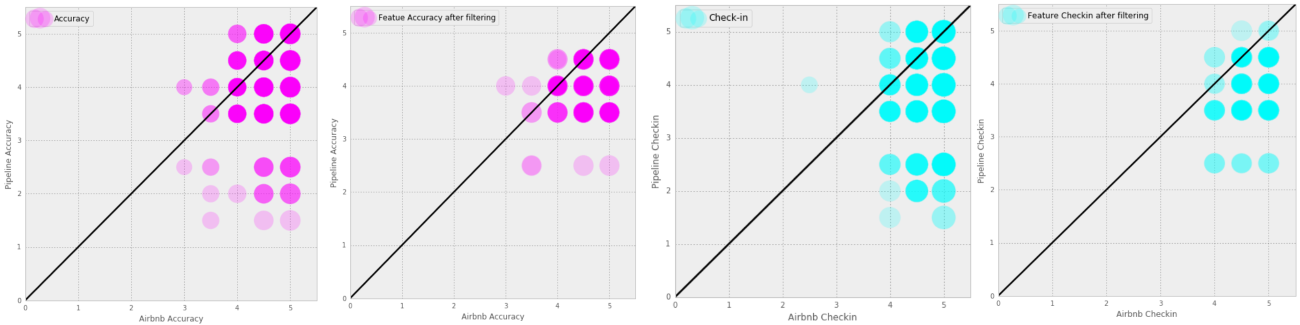
\includegraphics[height=0.21\textheight]{accuracy_checkin}
	\caption{RMSE per feature before and after setting the condition}
	\label{fig:6.6}
\end{figure}
In the case of feature level, it looks like the impact of conditioning the number of reviews per feature is more significant. The analysis showed that 16.5\%  of the listings do not have the sufficient number of reviews to generate a score in feature level. Table \ref{res4} shows the RMSE of differences between Airbnb and the pipeline, before and after setting the condition of having 3 reviews mentioning each feature of the listing. From the table, we see that the change is quite significant for \textit{Accuracy} and \textit{Check-in}, which aligns with the features with the smallest number of reviews, meaning that all the values produced from less than 3 reviews are omitted. Figure \ref{fig:6.6} shows how the distribution of the combinations changes after setting the condition for these two features. It is clearly seen that conditioning the number of reviews per feature makes the analysis more reliable and removes biggest the outliers. However, the phenomenon of having higher Airbnb values than the pipeline persist. This means that that feature-based opinion mining of reviews is particularly important, because  text reviews reveal hidden knowledge for features, which is not captured by the Airbnb feature rating system. The details of this analysis and the cases of other features can be found in Appendix. 
%
%
%
\section{Reducing the bias of Airbnb system}
In this chapter, we repeatedly have pointed out the systematic tendency of Airbnb ratings to be higher than the ratings generated by text review, as it is also suggested earlier in the literature \cite{fradkin2016bias, pavlou2006institutional, pavlou2006nature} and seen in Figure \ref{fig:6.8}. Up to here, we have seen that the RMSE of overall scores is 0.675 and it is not caused from an error of the pipeline in isolated cases. 
Figure \ref{fig:6.7} shows the distribution of sentiment scores of pipeline when evaluated by humans. In this distribution we see that there is no tendency of the pipeline to produce higher or lower sentiment scores, in contrast to Airbnb values, visualized in Figure \ref{fig:6.8}. Furthermore, the evaluation of the pipeline produced the exact average rating, mode and median as humans did. Therefore, the pipeline estimation of average values is considered highly accurate and representative of the real average ratings of the listings. The mean difference between Airbnb values and those produced by the pipeline is 0.57 stars, for simplicity reasons we round it to half a star. In order to prove the systematic tendency of Airbnb values to be higher than the one retrieved from text, all the Airbnb ratings are shifted with -0.5 stars. This action produces a set of new Airbnb ratings. The RMSE of two samples in this new situation equals 0.357, a significant reduction of almost 50\% from the initial value. Thus, we can conclude that a reduction of Airbnb values with half a star, which consider both manual ratings in the system and the text reviews, will produce better rating scores in the system.
\begin{figure}
\begin{minipage}{7cm}
\center
	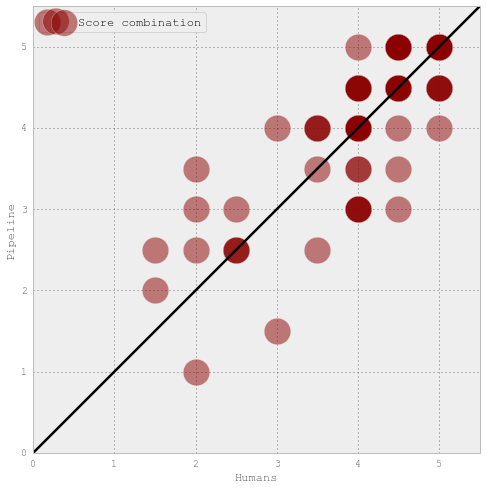
\includegraphics[height=0.32\textheight]{vaderhumans}
	\centering \caption{ Distribution of VADER and human scores from evaluation}
	\label{fig:6.7}
\end{minipage}
\hspace{2cm}
\begin{minipage}{7cm}
\centering
    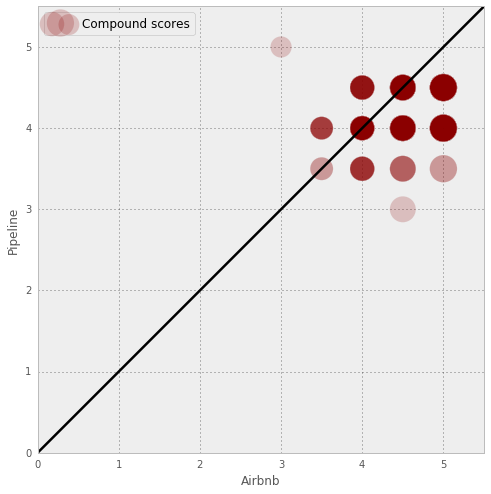
\includegraphics[height=0.32\textheight]{pipelineairbnb}
	\caption{Distribution of VADER and Airbnb scores}
	\label{fig:6.8}
\end{minipage}
\end{figure}